% questions.tex —— 2000 年·全国旧课程卷·文科 · 题目内容片段（无答案）
% 由 tools/generate_projects.py 依来源总账自 2000/2000_数学真题_全国旧课程文_试题.md 生成，勿手改（改源 MD 后重跑）


\gkpart{文科数学}

\begin{gktip}
\textbf{来源说明}：本题面依据固定源 PDF《2000 普通高等学校招生考试（旧课程卷文）》逐题转录。固定源为 2 页 A3 横向题面，原卷印刷页码 69–70；PDF 不含答案或解析页，下列答案和解析由本库独立推导，不声称代表官方发布版本。

\textbf{图形说明}：第 5、12、16、19、21、22 题的原卷图形关系重绘为 TikZ/PGFPlots 矢量图。图形标记所指的 PNG 不随仓库保存。
\end{gktip}

\gkpart{一、选择题}

\begin{question}
\gkti{1}设集合 $A=\{x\mid x\in\mathbb Z\text{ \text{且} }-10\le x\le-1\}$，$B=\{x\mid x\in\mathbb Z\text{ \text{且} }|x|\le5\}$，则 $A\cup B$ 中的元素个数是\mbox{（　　）}

（A）11　　（B）10　　（C）16　　（D）15

\end{question}
\begin{question}
\gkti{2}在复平面内，把复数 $3-\sqrt3\,i$ 对应的向量按顺时针方向旋转 $\dfrac\pi3$，所得向量对应的复数是\mbox{（　　）}

（A）$2\sqrt3$　　（B）$-2\sqrt3\,i$　　（C）$\sqrt3-3i$　　（D）$3+\sqrt3\,i$

\end{question}
\begin{question}
\gkti{3}一个长方体共一顶点的三个面的面积分别是 $\sqrt2$、$\sqrt3$、$\sqrt6$，这个长方体对角线的长是\mbox{（　　）}

（A）$2\sqrt3$　　（B）$3\sqrt2$　　（C）6　　（D）$\sqrt6$

\end{question}
\begin{question}
\gkti{4}已知 $\sin\alpha>\sin\beta$，那么下列命题成立的是\mbox{（　　）}

（A）若 $\alpha$、$\beta$ 是第一象限角，则 $\cos\alpha>\cos\beta$

（B）若 $\alpha$、$\beta$ 是第二象限角，则 $\tan\alpha>\tan\beta$

（C）若 $\alpha$、$\beta$ 是第三象限角，则 $\cos\alpha>\cos\beta$

（D）若 $\alpha$、$\beta$ 是第四象限角，则 $\tan\alpha>\tan\beta$

\Needspace{0.4\textheight}
\end{question}
\begin{question}
\gkti{5}函数 $y=-x\cos x$ 的部分图象是\mbox{（　　）}
\nopagebreak[4]
\begin{center}% 2000 年全国旧课程卷文科第 5 题：y=-x cos x 的四个图象选项
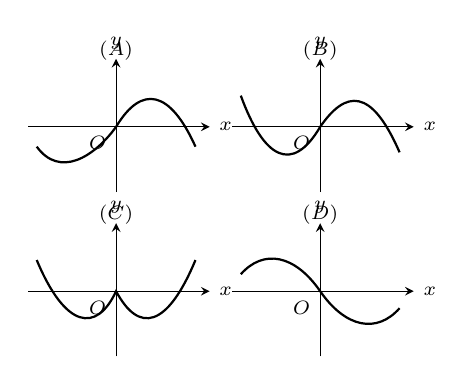
\begin{tikzpicture}[>=stealth, scale=0.72]
  \begin{scope}
    \node[font=\scriptsize] at (0,1.35) {$(A)$};
    \draw[->] (-1.55,0)--(1.65,0) node[right, font=\scriptsize] {$x$};
    \draw[->] (0,-1.15)--(0,1.2) node[above, font=\scriptsize] {$y$};
    \draw[thick] (-1.4,-0.35) .. controls (-1.0,-0.9) and (-0.4,-0.55) .. (0,0)
      .. controls (0.45,0.75) and (0.95,0.65) .. (1.4,-0.35);
    \node[below left, font=\scriptsize] at (0,0) {$O$};
  \end{scope}

  \begin{scope}[xshift=3.6cm]
    \node[font=\scriptsize] at (0,1.35) {$(B)$};
    \draw[->] (-1.55,0)--(1.65,0) node[right, font=\scriptsize] {$x$};
    \draw[->] (0,-1.15)--(0,1.2) node[above, font=\scriptsize] {$y$};
    \draw[thick] (-1.4,0.55) .. controls (-1.0,-0.55) and (-0.5,-0.85) .. (0,0)
      .. controls (0.45,0.65) and (0.9,0.7) .. (1.4,-0.45);
    \node[below left, font=\scriptsize] at (0,0) {$O$};
  \end{scope}

  \begin{scope}[yshift=-2.9cm]
    \node[font=\scriptsize] at (0,1.35) {$(C)$};
    \draw[->] (-1.55,0)--(1.65,0) node[right, font=\scriptsize] {$x$};
    \draw[->] (0,-1.15)--(0,1.2) node[above, font=\scriptsize] {$y$};
    \draw[thick] (-1.4,0.55) .. controls (-0.9,-0.65) and (-0.35,-0.75) .. (0,0)
      .. controls (0.4,-0.75) and (0.9,-0.65) .. (1.4,0.55);
    \node[below left, font=\scriptsize] at (0,0) {$O$};
  \end{scope}

  \begin{scope}[xshift=3.6cm,yshift=-2.9cm]
    \node[font=\scriptsize] at (0,1.35) {$(D)$};
    \draw[->] (-1.55,0)--(1.65,0) node[right, font=\scriptsize] {$x$};
    \draw[->] (0,-1.15)--(0,1.2) node[above, font=\scriptsize] {$y$};
    \draw[thick] (-1.4,0.3) .. controls (-1.0,0.75) and (-0.45,0.65) .. (0,0)
      .. controls (0.45,-0.65) and (1.0,-0.75) .. (1.4,-0.3);
    \node[below left, font=\scriptsize] at (0,0) {$O$};
  \end{scope}
\end{tikzpicture}
\end{center}
\nopagebreak[4]
\end{question}
\begin{question}
\gkti{6}《中华人民共和国个人所得税法》规定，公民全月工资、薪金所得不超过 800 元的部分不必纳税，超过 800 元的部分为全月应纳税所得额，此项税款按下表分段累进计算：

\begin{center}
\begin{tabular}{lr}
\toprule
全月应纳税所得额 & 税率 \\
\midrule
不超过 500 元的部分 & 5\% \\
超过 500 元至 2000 元的部分 & 10\% \\
超过 2000 元至 5000 元的部分 & 15\% \\
$\cdots$ & $\cdots$ \\
\bottomrule
\end{tabular}
\end{center}

某人一月份交纳此项税款 26.78 元，则他的当月工资、薪金所得介于\mbox{（　　）}

（A）800–900 元　　（B）900–1200 元

（C）1200–1500 元　　（D）1500–2800 元

\end{question}
\begin{question}
\gkti{7}若 $a>b>1$，$P=\sqrt{\lg a\cdot\lg b}$，$Q=\dfrac12(\lg a+\lg b)$，$R=\lg\dfrac{a+b}{2}$，则\mbox{（　　）}

（A）$R<P<Q$　　（B）$P<Q<R$　　（C）$Q<P<R$　　（D）$P<R<Q$

\end{question}
\begin{question}
\gkti{8}已知两条直线 $l_1:y=x$，$l_2:ax-y=0$，其中 $a$ 为实数。当这两条直线的夹角在 $\left(0,\dfrac\pi{12}\right)$ 内变动时，$a$ 的取值范围是\mbox{（　　）}

（A）$\left(0,1\right)$　　（B）$\left(\dfrac{\sqrt3}{3},\sqrt3\right)$

（C）$\left(\dfrac{\sqrt3}{3},1\right)\cup\left(1,\sqrt3\right)$　　（D）$\left(1,\sqrt3\right)$

\end{question}
\begin{question}
\gkti{9}一个圆柱的侧面展开图是一个正方形，这个圆柱的全面积与侧面积的比是\mbox{（　　）}

（A）$\dfrac{1+2\pi}{2\pi}$　　（B）$\dfrac{1+4\pi}{4\pi}$　　（C）$\dfrac{1+2\pi}{\pi}$　　（D）$\dfrac{1+4\pi}{2\pi}$

\end{question}
\begin{question}
\gkti{10}过原点的直线与圆 $x^2+y^2+4x+3=0$ 相切，若切点在第三象限，则该直线的方程是\mbox{（　　）}

（A）$y=\sqrt3x$　　（B）$y=-\sqrt3x$　　（C）$y=\dfrac{\sqrt3}{3}x$　　（D）$y=-\dfrac{\sqrt3}{3}x$

\end{question}
\begin{question}
\gkti{11}过抛物线 $y=ax^2\ (a>0)$ 的焦点 $F$ 作一直线交抛物线于 $P$、$Q$ 两点，若线段 $PF$ 与 $FQ$ 的长分别是 $p$、$q$，则 $\dfrac1p+\dfrac1q$ 等于\mbox{（　　）}

（A）$2a$　　（B）$\dfrac1{2a}$　　（C）$4a$　　（D）$\dfrac4a$

\Needspace{0.4\textheight}
\end{question}
\begin{question}
\gkti{12}如图，$OA$ 是圆锥底面中心 $O$ 到母线的垂线，$OA$ 绕轴旋转一周所得曲面将圆锥分成体积相等的两部分，则母线与轴的夹角为\mbox{（　　）}
\nopagebreak[4]
\begin{center}% 2000 年全国旧课程卷文科第 12 题：圆锥轴截面与 OA
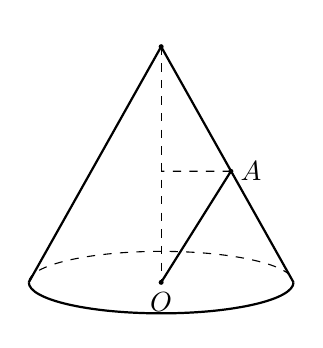
\begin{tikzpicture}[>=stealth, scale=0.82]
  \coordinate (V) at (0,3.65);
  \coordinate (O) at (0,0);
  \coordinate (L) at (-2.05,0);
  \coordinate (R) at (2.05,0);
  \coordinate (A) at (1.08,1.72);
  \draw[thick] (V)--(L) (V)--(R);
  \draw[thick] (L) arc (180:360:2.05 and 0.48);
  \draw[dashed] (L) arc (180:0:2.05 and 0.48);
  \draw[dashed] (V)--(O);
  \draw[thick] (O)--(A);
  \draw[dashed] (A)--(0,1.72);
  \fill (V) circle (1.1pt);
  \fill (O) circle (1.1pt) node[below] {$O$};
  \fill (A) circle (1.1pt) node[right] {$A$};
  \node[above] at (V) { };
\end{tikzpicture}
\end{center}
\nopagebreak[4]
（A）$\arccos\dfrac1{\sqrt[3]{2}}$　　（B）$\arccos\dfrac12$　　（C）$\arccos\dfrac1{\sqrt2}$　　（D）$\arccos\dfrac1{\sqrt[4]{2}}$

\end{question}
\gkpart{二、填空题}

\begin{question}
\gkti{13}乒乓球队的 10 名队员中有 3 名主力队员，派 5 名参加比赛，3 名主力队员要安排在第一、三、五位置，其余 7 名队员选 2 名安排在第二、四位置，那么不同的出场安排共有\gkblank{}种（用数字作答）。

\end{question}
\begin{question}
\gkti{14}椭圆 $\dfrac{x^2}{9}+\dfrac{y^2}{4}=1$ 的焦点 $F_1,F_2$，点 $P$ 为其上的动点，当 $\angle F_1PF_2$ 为钝角时，点 $P$ 横坐标的取值范围是\gkblank{}。

\end{question}
\begin{question}
\gkti{15}设 $\{a_n\}$ 是首项为 1 的正项数列，且

\nopagebreak[4]
\[
(n+1)a_{n+1}^2-na_n^2+a_{n+1}a_n=0
\qquad(n=1,2,3,\ldots),
\]

则它的通项公式是 $a_n=$\gkblank{}。

\Needspace{0.4\textheight}
\end{question}
\begin{question}
\gkti{16}如图，$E$、$F$ 分别为正方体面 $ADD_1A_1$、面 $BCC_1B_1$ 的中心，则四边形 $BFD_1E$ 在该正方体的面上的射影可能是\gkblank{}。（要求：把可能的图序号都填上）
\nopagebreak[4]
\begin{center}% 2000 年全国旧课程卷文科第 16 题：正方体内四边形投影的可能图形
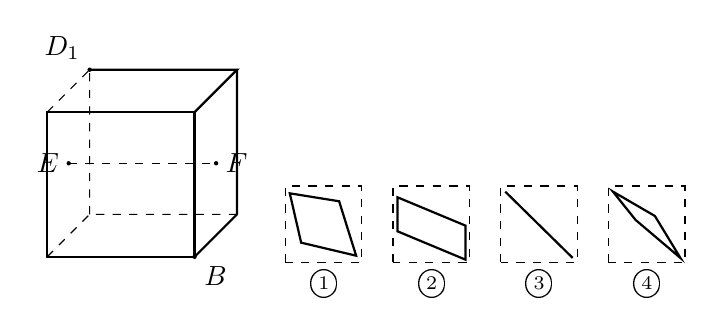
\begin{tikzpicture}[>=stealth, scale=0.72]
  \coordinate (A) at (0,0);
  \coordinate (B) at (2.6,0);
  \coordinate (C) at (3.35,0.75);
  \coordinate (D) at (0.75,0.75);
  \coordinate (A1) at (0,2.55);
  \coordinate (B1) at (2.6,2.55);
  \coordinate (C1) at (3.35,3.3);
  \coordinate (D1) at (0.75,3.3);
  \coordinate (E) at (0.38,1.65);
  \coordinate (F) at (2.98,1.65);

  \draw[thick] (A)--(B)--(B1)--(A1)--cycle;
  \draw[thick] (B1)--(C1)--(D1);
  \draw[dashed] (A)--(D)--(C) (D)--(D1) (A1)--(D1);
  \draw[thick] (B)--(C) (C)--(C1);
  \draw[dashed] (E)--(F);
  \fill (B) circle (1.1pt) node[below right] {$B$};
  \fill (D1) circle (1.1pt) node[above left] {$D_1$};
  \fill (E) circle (1.1pt) node[left] {$E$};
  \fill (F) circle (1.1pt) node[right] {$F$};

  \begin{scope}[xshift=4.2cm,yshift=-0.1cm]
    \draw[dashed] (0,0) rectangle (1.35,1.35);
    \draw[thick] (0.08,1.22)--(0.95,1.08)--(1.25,0.12)--(0.28,0.35)--cycle;
    \node[below] at (0.68,-0.08) {\textcircled{\scriptsize 1}};
  \end{scope}
  \begin{scope}[xshift=6.1cm,yshift=-0.1cm]
    \draw[dashed] (0,0) rectangle (1.35,1.35);
    \draw[thick] (0.08,1.15)--(0.08,0.55)--(1.28,0.05)--(1.28,0.65)--cycle;
    \node[below] at (0.68,-0.08) {\textcircled{\scriptsize 2}};
  \end{scope}
  \begin{scope}[xshift=8.0cm,yshift=-0.1cm]
    \draw[dashed] (0,0) rectangle (1.35,1.35);
    \draw[thick] (0.08,1.25)--(1.27,0.08);
    \node[below] at (0.68,-0.08) {\textcircled{\scriptsize 3}};
  \end{scope}
  \begin{scope}[xshift=9.9cm,yshift=-0.1cm]
    \draw[dashed] (0,0) rectangle (1.35,1.35);
    \draw[thick] (0.08,1.25)--(0.48,0.75)--(1.27,0.08)--(0.82,0.82)--cycle;
    \node[below] at (0.68,-0.08) {\textcircled{\scriptsize 4}};
  \end{scope}
\end{tikzpicture}
\end{center}
\nopagebreak[4]
\end{question}
\begin{question}
\gkti{17}已知函数

\nopagebreak[4]
\[
y=\sqrt3\sin x+\cos x,\qquad x\in\mathbb R\text{。}
\]

（1） 当函数 $y$ 取得最大值时，求自变量 $x$ 的集合；

（2） 该函数的图象可由 $y=\sin x\ (x\in\mathbb R)$ 的图象经过怎样的平移和伸缩变换得到？

\end{question}
\gkpart{三、解答题}

\begin{question}
\gkti{18}设 $\{a_n\}$ 为等差数列，$S_n$ 为数列 $\{a_n\}$ 的前 $n$ 项和，已知 $S_7=7$，$S_{15}=75$，$T_n$ 为数列 $\left\{\dfrac{S_n}{n}\right\}$ 的前 $n$ 项和，求 $T_n$。

\Needspace{0.4\textheight}
\end{question}
\begin{question}
\gkti{19}如图，已知平行六面体 $ABCD-A_1B_1C_1D_1$ 的底面 $ABCD$ 是菱形，且

\nopagebreak[4]
\[
\angle C_1CB=\angle C_1CD=\angle BCD=60^\circ\text{。}
\]

（1） 证明：$C_1C\perp BD$；

（2） 当 $\dfrac{CD}{CC_1}$ 的值为多少时，能使 $A_1C\perp$ 平面 $C_1BD$？请给出证明。
\nopagebreak[4]
\begin{center}% 2000 年全国旧课程卷文科第 19 题：平行六面体 ABCD-A_1B_1C_1D_1
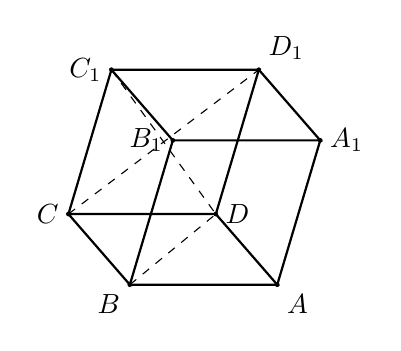
\begin{tikzpicture}[>=stealth, scale=0.78]
  \coordinate (A) at (3.4,0);
  \coordinate (B) at (1.0,0);
  \coordinate (C) at (0,1.15);
  \coordinate (D) at (2.4,1.15);
  \coordinate (A1) at (4.1,2.35);
  \coordinate (B1) at (1.7,2.35);
  \coordinate (C1) at (0.7,3.5);
  \coordinate (D1) at (3.1,3.5);

  \draw[thick] (A)--(B)--(C)--(D)--cycle;
  \draw[thick] (A1)--(B1)--(C1)--(D1)--cycle;
  \draw[thick] (A)--(A1) (B)--(B1) (C)--(C1) (D)--(D1);
  \draw[dashed] (C1)--(D) (B)--(D) (C)--(D1);

  \fill (A) circle (1.1pt) node[below right] {$A$};
  \fill (B) circle (1.1pt) node[below left] {$B$};
  \fill (C) circle (1.1pt) node[left] {$C$};
  \fill (D) circle (1.1pt) node[right] {$D$};
  \fill (A1) circle (1.1pt) node[right] {$A_1$};
  \fill (B1) circle (1.1pt) node[left] {$B_1$};
  \fill (C1) circle (1.1pt) node[left] {$C_1$};
  \fill (D1) circle (1.1pt) node[above right] {$D_1$};
\end{tikzpicture}
\end{center}
\nopagebreak[4]
\end{question}
\begin{question}
\gkti{20}设函数 $f(x)=\sqrt{x^2+1}-ax$，其中 $a>0$。

（1） 解不等式 $f(x)\le1$；

（2） 证明：当 $a\ge1$ 时，函数 $f(x)$ 在区间 $[0,+\infty)$ 上是单调函数。

\Needspace{0.4\textheight}
\end{question}
\begin{question}
\gkti{21}某蔬菜基地种植西红柿，由历年市场行情得知，从二月一日起的 300 天内，西红柿市场售价与上市时间的关系用图一的一条折线表示；西红柿的种植成本与上市时间的关系用图二的抛物线段表示。

（1） 写出图一表示的市场售价与时间的函数关系式 $p=f(t)$；写出图二表示的种植成本与时间的函数关系式 $Q=g(t)$；

（2） 认定市场售价减去种植成本为纯收益，问何时上市的西红柿纯收益最大？

注：市场售价和各种植成本的单位：元/$10^2\mathrm{kg}$，时间单位：天。
\nopagebreak[4]
\begin{center}% 2000 年全国旧课程卷文科第 21 题：市场售价与种植成本图象
\begin{tikzpicture}[>=stealth, scale=0.78]
  \begin{scope}
    \draw[->] (0,0)--(3.55,0) node[right] {$t$};
    \draw[->] (0,0)--(0,3.65) node[above] {$P$};
    \draw[thick] (0,3.0)--(2.0,1.0)--(3.0,3.0);
    \draw[dashed] (0,3.0)--(3.0,3.0) (0,1.0)--(2.0,1.0)
      (2.0,0)--(2.0,1.0) (3.0,0)--(3.0,3.0);
    \node[left, font=\scriptsize] at (0,3.0) {300};
    \node[left, font=\scriptsize] at (0,1.0) {100};
    \node[below, font=\scriptsize] at (2.0,0) {200};
    \node[below, font=\scriptsize] at (3.0,0) {300};
    \node[below] at (1.5,-0.42) {图一};
  \end{scope}
  \begin{scope}[xshift=4.35cm]
    \draw[->] (0,0)--(3.55,0) node[right] {$t$};
    \draw[->] (0,0)--(0,3.65) node[above] {$Q$};
    \draw[thick, domain=0:3, samples=80]
      plot (\x,{1+(\x-1.5)^2/2});
    \draw[dashed] (0,1)--(3,1) (0,1.5)--(0.5,1.5) (0,1.5)--(2.5,1.5)
      (0.5,0)--(0.5,1.5) (1.5,0)--(1.5,1) (2.5,0)--(2.5,1.5);
    \node[left, font=\scriptsize] at (0,3.0) {300};
    \node[left, font=\scriptsize] at (0,2.5) {250};
    \node[left, font=\scriptsize] at (0,1.5) {150};
    \node[left, font=\scriptsize] at (0,1.0) {100};
    \node[below, font=\scriptsize] at (0.5,0) {50};
    \node[below, font=\scriptsize] at (1.5,0) {150};
    \node[below, font=\scriptsize] at (2.5,0) {250};
    \node[below] at (1.5,-0.42) {图二};
  \end{scope}
\end{tikzpicture}
\end{center}
\nopagebreak[4]
\Needspace{0.4\textheight}
\end{question}
\begin{question}
\gkti{22}如图，已知梯形 $ABCD$ 中 $|AB|=2|CD|$，点 $E$ 分有向线段 $\overline{AC}$ 所成的比为 $\lambda$，双曲线过 $C,D,E$ 三点，且以 $A\text{、}B$ 为焦点，当 $\dfrac23\le\lambda\le\dfrac34$ 时，求双曲线离心率 $e$ 的取值范围。
\nopagebreak[4]
\begin{center}% 2000 年全国旧课程卷文科第 22 题：梯形、分点与双曲线
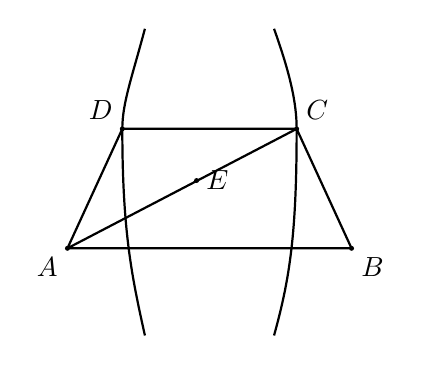
\begin{tikzpicture}[>=stealth, scale=0.82]
  \coordinate (A) at (0,0);
  \coordinate (B) at (4.4,0);
  \coordinate (D) at (0.85,1.85);
  \coordinate (C) at (3.55,1.85);
  \coordinate (E) at (2.0,1.05);

  \draw[thick] (A)--(B)--(C)--(D)--cycle;
  \draw[thick] (A)--(C);
  \draw[thick] (1.2,3.4) .. controls (1.0,2.65) and (0.85,2.25) .. (0.85,1.85);
  \draw[thick] (3.2,3.4) .. controls (3.45,2.7) and (3.55,2.25) .. (3.55,1.85);
  \draw[thick] (1.2,-1.35) .. controls (1.0,-0.45) and (0.85,0.25) .. (0.85,1.85);
  \draw[thick] (3.2,-1.35) .. controls (3.45,-0.45) and (3.55,0.25) .. (3.55,1.85);

  \fill (A) circle (1.1pt) node[below left] {$A$};
  \fill (B) circle (1.1pt) node[below right] {$B$};
  \fill (C) circle (1.1pt) node[above right] {$C$};
  \fill (D) circle (1.1pt) node[above left] {$D$};
  \fill (E) circle (1.1pt) node[right] {$E$};
\end{tikzpicture}
\end{center}
\nopagebreak[4]

\end{question}